% ===== STEP 2: Define Search Strategy =====
% This section covers:
% - Search strategy development
% - Documentation of search process

\begin{figure*}[th]
	\centering
	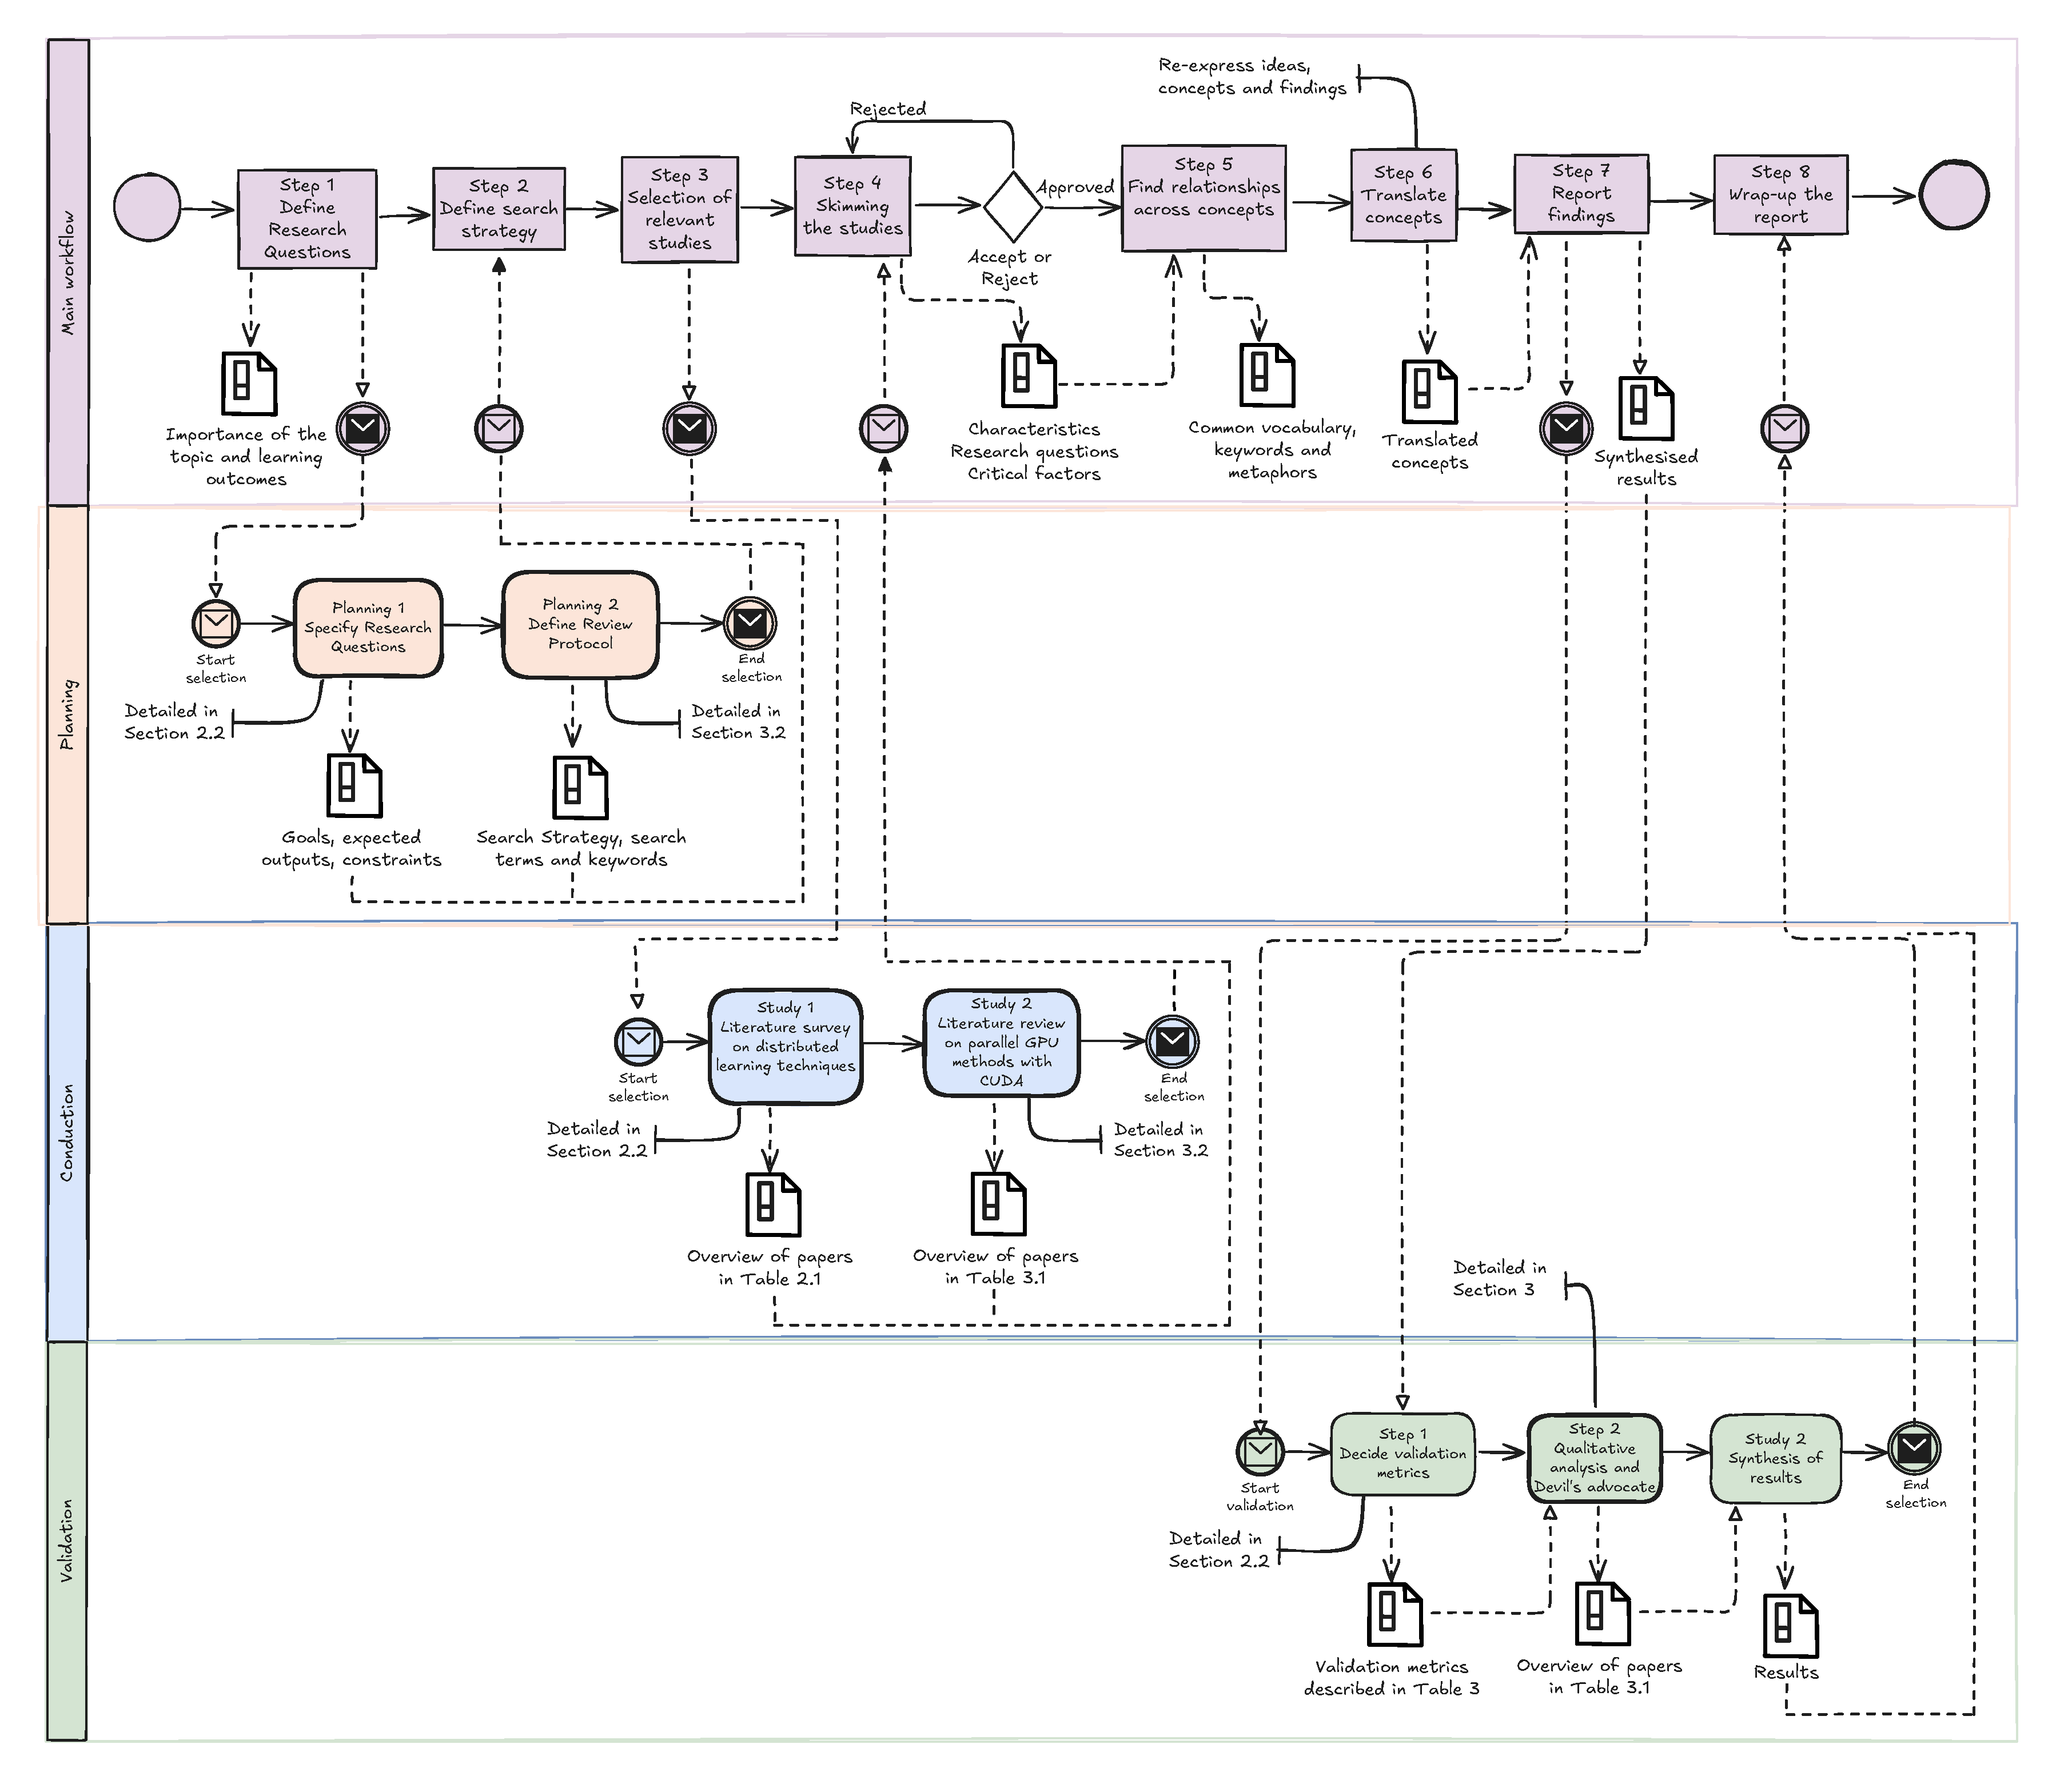
\includegraphics[width=\linewidth]{figures/workflow2}
	\caption{Systematic review workflow showing the main steps, documentation artifacts, and validation processes.
		The workflow is divided into three main phases: main workflow (top), studies selection (middle), and
		validation (bottom). Dashed lines indicate documentation and communication flows. Adapted from \cite{dos_santos_sustainable_2024}.}
	\label{fig:workflow}
\end{figure*}

\section{Related Work}

\TODO{Reference the related work on survying the present methods both in DDL and CUDA}

Related work focuses on techniques and algorithms for training deep learning models across multiple
machines \cite{dehghani_distributed_2023, chahal_hitchhikers_2018, berloco_systematic_2022}. These
sources explore various aspects of DDL, such as parallelization techniques and communication
methods. However, our contribution emphasizes the connection between DDL and GPU programming with
CUDA. Furthermore, this study details the main libraries for DDL and GPU programming. We will also
provide practical guidance on running a small neural network in CUDA and facilitating PyTorch
Distributed Data Parallel (DDP) programming using Docker, addressing a practical implementation gap
not covered in the previous work. \TODO{Highlight related surveys concerning CUDA}

This study follows primarily the guidelines described in \cite{keele_systematic_2007}, however
advice for conducting the review is synthesized from a wider range of related articles
\cite{brereton_lessons_2007-1,kitchenham_procedures_nodate,budgen_reporting_2018,dos_santos_sustainable_2024}.

Distributed training of neural networks has become essential for modern deep learning applications
due to increasing model complexity and dataset sizes \cite{chahal_hitchhikers_2018}. The main
approaches for distributing neural network training can be categorized into several key strategies
\cite{dehghani_distributed_2023}:

\begin{itemize}
	\item \textbf{Data Parallelism:}
	      The dataset is divided across multiple nodes, with each node training a complete copy of the
	      model on its portion of data. Gradients from all nodes are then combined to update the model parameters.
	      This approach can be implemented either synchronously (all nodes wait for each other) or asynchronously (nodes work independently).

	\item \textbf{Model Parallelism:}
	      The neural network model itself is divided across different nodes, with each node responsible
	      for computing a specific portion of the model architecture. This strategy is particularly useful
	      when the model is too large to fit on a single machine.

	\item \textbf{Pipeline Parallelism:}
	      The training process is divided into sequential stages, similar to an assembly line,
	      where the output of one stage becomes the input for the next. This allows different parts
	      of the model to train simultaneously while maintaining dependencies.

	\item \textbf{Hybrid Parallelism:}
	      This approach combines multiple parallelization strategies to optimize training efficiency.
	      For example, model parallelism might be used to distribute a large model across GPUs, while
	      data parallelism is applied to each model segment.
\end{itemize}

These approaches can be further enhanced through techniques such as gradient compression, mixed
precision training, and tensor fusion \cite{dehghani_distributed_2023}. The choice of specific
techniques depends on factors including model architecture, available hardware, and training
requirements. For a comprehensive review of these techniques and their implementations, readers are
referred to \cite{chahal_hitchhikers_2018}.

\section{Review Protocol}
\label{sec:protocol}

The review protocol is a key component of the review process, as it represents the planning phase
that enables the conduction of a review that is both transparent and replicable. To ensure this,
the process is documented and most of the resulting artifacts are present in the text and in the
Appendix.

% Now detail Step 1 content
The workflow is shown in Figure \ref{fig:workflow} where the key phases are annotated as: Planning
the Review (W1, W2), Conducting the Review (W3, W4, W5), and Reporting the Review (W6, W7, W8).

Parts of the review protocol have already been defined, such as the incentive for conducting a
systematic review in Section \ref{sec:importance_of_topic}.

\subsection{P1. Research Questions}
\label{sec:research_questions}
Following the workflow diagram (Step P1), the initial research questions described in Section
\ref{sec:initial_research_questions} are expanded as a result of iterating over the review protocol
and investigating some of the known information sources.

\begin{itemize}
	\item What are the different techniques for parallelising deep learning models and data
	      \cite{berloco_systematic_2022, ben-nun_demystifying_2020, langer_distributed_2020}?
	      % NOTE \item How do parameter update strategies impact distributed deep learning systems (e.g., Parameter Server and decentralised approaches) \cite{ben-nun_demystifying_2020,berloco_systematic_2022,langer_distributed_2020}?
	\item How is stochastic gradient descent (SGD) computed in distributed environments
	      \cite{berloco_systematic_2022,ben-nun_demystifying_2020,langer_distributed_2020,verbraeken_survey_2021}? % NOTE and what are the associated challenges 
	\item What are the key frameworks currently available for implementing DDL, and how do their features
	      compare \cite{berloco_systematic_2022}?
\end{itemize}

Concerning GPU parallelization, the following questions : \TODO{Could be improved}
\begin{itemize}
	\item How does CUDA enable data parallelization on single-machine GPUs?
	\item What are key frameworks for implementing CUDA parallelization?
	\item What similarities are there between CUDA and DDL techniques?
\end{itemize}

Of particular interest is to check for intertwined connections between the two topics:
\begin{itemize}
	\item In what ways are the techniques used in DDL also useful in GPU parallelization?
\end{itemize}

The questions play a key role in guiding the search strategy, data extraction process and results
synthesis phases.

% The workflow also shows the documentation artifacts and validation processes that occur throughout the review, ensuring rigor and transparency.

\subsection{P2. Search Strategy}

% Moved the explanation of the phases here
% A systematic literature review involves several discrete activities. Existing guidelines for systematic reviews have slightly different suggestions about the number and order of activities. This document summarises the stages in a systematic review into three main phases: Planning the Review, Conducting the Review, Reporting the Review.

As suggested by \cite{keele_systematic_2007}, search strategy is used (P2 in Step
\ref{fig:workflow}).

\textbf{Search Strategy.}
The search process includes a manual search of specific citation databases that include conference
proceedings and journal papers. The nominated databases are shown in Table \ref{tab:databases}. A
number of search strings were constructed using relevant terms based on the research questions.

The search was restricted to papers published between $\yearstartcuda$ and $\yearendcuda$ for the
CUDA task and between $\yearstartddl$ and $\yearendddl$ for the DDL task. The former start year
($\yearstartcuda$) was chosen as the baseline as this was the year when AlexNet was published (the
key paper which started the deep learning revolution). The latter start year ($\yearstartddl$) was
chosen as a result of an initial survey of the literature that determined when the first papers in
distributed deep learning started to appear. \TODO{To review}

\begin{table}[htbp]
	\centering
	\caption{Search Engines Used}
	\label{tab:databases}
	\begin{tabular}{|l|r|}
		\hline
		\textbf{Search Engine} & \textbf{Number of uses} \\
		\hline
		IEEExplore             & 33                      \\
		ACM                    & 30                      \\
		ScienceDirect          & 24                      \\
		Web of Science         & 19                      \\
		Google Scholar         & 18                      \\
		SpringerLink           & 17                      \\
		Scopus                 & 14                      \\
		Compendex              & 11                      \\
		CiteSeer               & 5                       \\
		\hline
	\end{tabular}
\end{table}

% ===== STEP 3: Selection of Relevant Studies =====
% This section details:
% - Study 1: Distributed learning techniques
% - Study 2: CUDA implementations
\subsection{Study Selection Framework}
\label{sec:study-selection}

% Combined "Purpose," "Scope," and "Relationship Between Study Types"
This section defines the aims and scope of the review, clarifying the types of studies to be
included and the rationale for exploring distributed learning and CUDA implementations together.
The specific objectives of the review are aligned with the associated research questions to provide
a clear focus. The boundaries of the review concern the types of distributed learning techniques
and CUDA implementations considered, with a time period between 2015 and 2022 to ensure currency.
The review includes studies focusing on the design and analysis of distributed learning algorithms
and those focusing on CUDA-based parallel implementations to understand the translation of
theoretical aspects into practical implementations. This approach allows for the exploration of
patterns and challenges in mapping distributed algorithms onto parallel architectures
\TODO{Different topics explored together}.

\subsubsection{Distributed Learning Techniques Review}
The review will focus on distributed learning approaches, aligning with "Study 1" in Figure
\ref{fig:workflow}, with the following considerations:
\begin{itemize}
	\item Types of algorithms including \textbf{data parallelism, model parallelism, and asynchronous
		      Stochastic Gradient Descent (SGD)} \cite{ben-nun_demystifying_2020,langer_distributed_2020}.
	\item Different distributed architectures including parameter servers and peer-to-peer systems
	      \cite{verbraeken_survey_2021,ben-nun_demystifying_2020,langer_distributed_2020}.
	\item Specific machine learning models such as neural networks and support vector machines.
\end{itemize}

\subsubsection{CUDA-based Parallel Implementation Review}
For CUDA implementations, the review will consider aspects relevant to "Study 2" in Figure
\ref{fig:workflow}:
\begin{itemize}
	\item Implementation of distributed methods on NVIDIA GPUs using the CUDA framework
	\item Different CUDA libraries and architectures
	\item Specific hardware considerations including GPUs and Tensor Processing Units (TPUs)
\end{itemize}

\subsubsection{Justification for Inclusion}
Both distributed learning techniques and CUDA implementation studies will be included to provide a
complete picture of the current state-of-the-art research in the area. By including both study
types, a deeper understanding of both theoretical approaches and implementation techniques for
practical applications can be reached.

\subsection{Preliminary Protocol Development}
This systematic review follows the guidelines proposed by Kitchenham and Charters for software
engineering research. The preliminary review protocol was developed to establish the foundation for
the steps visualized in Figure \ref{fig:workflow}, particularly in the initial stages. An overview
of the papers included after the initial selection phase (corresponding to the output of the
"Studies Selection" phase in Figure \ref{fig:workflow}) will be presented in Table 2.1.

\subsubsection{Background and Rationale}
This section provides the necessary context for the review, outlining the research gaps that will
be addressed \cite{ben-nun_demystifying_2020}. It explicitly states the need for a systematic
review of the current literature to address this gap and provide a focused analysis.

\subsubsection{Initial Search Strategy}
The initial search strategy involves combining keywords using Boolean and proximity operators to
generate search strings, based on the "Goals, expected outputs, constraints, search terms and
keywords" documented as an input to Step 1 in Figure \ref{fig:workflow}. Databases like Scopus,
Google Scholar, and ACM Digital Library are selected for their coverage of computer science,
engineering, and applied mathematics literature. Studies published between 2015-2022 will be
considered to ensure recent advancements are included while maintaining a consistent period for
analysis.
\begin{itemize}
	\item \textbf{Search Terms:} Details of the search terms will be provided in Section \ref{sec:search_process_documentation}.
	\item \textbf{Database Justification:} Rationale for selecting specific databases is detailed in Section \ref{sec:search_process_documentation}.
	\item \textbf{Timeline:} The timeframe for including studies is 2015-2022.
\end{itemize}

\subsubsection{Preliminary Selection Criteria}
Preliminary criteria for inclusion will use specific examples such as ``studies that evaluate the
performance of synchronous distributed SGD in deep learning models'' rather than general terms like
``distributed computing'' \cite{ben-nun_demystifying_2020}. Preliminary quality thresholds will
ensure only high-quality studies are included in the final analysis. Specific inclusion and
exclusion criteria are detailed in Section \ref{sec:study-selection-criteria}.

\subsubsection{Initial Data Extraction Plan}
The following information will be extracted from each study:
\begin{itemize}
	\item Details of distributed systems \cite{ben-nun_demystifying_2020,langer_distributed_2020}:
	      \begin{enumerate}
		      \item Number of nodes
		      \item Communication network
		      \item Communication method
		      \item Topology
	      \end{enumerate}
	\item Machine learning algorithms and models used \cite{xing_strategies_2015}.
	\item Datasets and benchmarks \cite{ben-nun_demystifying_2020}.
	\item Performance metrics (training time, accuracy, speedup)
	      \cite{ben-nun_demystifying_2020,langer_distributed_2020,xing_strategies_2015}.
	\item CUDA implementation details (libraries, optimizations)
	      \cite{verbraeken_survey_2021,ben-nun_demystifying_2020,xing_strategies_2015}.
\end{itemize}
Further details on the data extraction strategy can be found in Section \ref{sec:data-extraction-strategy}.

\subsubsection{Quality Assessment Framework}
Preliminary quality assessment will use specific criteria to evaluate the validity and reliability
of methods, using established checklists from the literature \cite{ben-nun_demystifying_2020}. A
Likert scale will be used for a standardized approach. Detailed guidelines for reviewers will be
established to ensure consistency and prevent bias, as described further in Section
\ref{sec:quality-assessment-process}.
\begin{itemize}
	\item \textbf{Criteria:} Specific criteria are detailed in Section \ref{sec:quality-assessment-process}.
	\item \textbf{Scoring System:} A Likert scale will be used.
	\item \textbf{Guidelines:} Guidelines for reviewers are detailed in Section \ref{sec:quality-assessment-process}.
\end{itemize}

\subsubsection{Synthesis Approach}
The synthesis approach will involve meta-analysis where appropriate, using statistical analysis to
combine results from included studies with clearly defined methods
\cite{ben-nun_demystifying_2020}. Thematic synthesis will be used for narrative synthesis, allowing
an in-depth understanding of themes present in selected studies.
\begin{itemize}
	\item \textbf{Meta-analysis:} Details of the methods will be defined later.
	\item \textbf{Narrative synthesis:} Thematic synthesis will be employed.
\end{itemize}

\subsection{Search Process Documentation}
\label{sec:search_process_documentation}
This section provides an overview of our search strategy. Detailed search documentation, including exact search strings and results for each database, can be found in the supplementary materials (Section \ref{sec:search_strategy}).

\subsubsection{Search Strategy Overview}
Our search strategy combines terms from two main categories as shown in Table
\ref{tab:search_terms}. The number of articles retrieved from each database is presented in Table
\ref{tab:search_results}.

\begin{table*}[ht]
	\centering
	\caption{Number of Retrieved Articles by Database}
	\label{tab:search_results}
	\begin{tabular}{|l|c|c|c|}
		\hline
		\textbf{Database}   & \textbf{Initial Results} & \textbf{After Filtering} & \textbf{Final Selection} \\
		\hline
		Scopus              & XXX                      & XXX                      & XXX                      \\
		\hline
		Google Scholar      & XXX                      & XXX                      & XXX                      \\
		\hline
		ACM Digital Library & XXX                      & XXX                      & XXX                      \\
		\hline
		IEEE Xplore         & XXX                      & XXX                      & XXX                      \\
		\hline
		Science Direct      & XXX                      & XXX                      & XXX                      \\
		\hline
		arXiv               & XXX                      & XXX                      & XXX                      \\
		\hline
		\textbf{Total}      & XXX                      & XXX                      & XXX                      \\
		\hline
	\end{tabular}
\end{table*}

The complete search strings for each database, including any database-specific adaptations, are
documented in Section \ref{sec:search_strategy} of the supplementary materials.

\subsection{Study Selection Criteria}
\label{sec:study-selection-criteria}
This section specifies the detailed inclusion and exclusion criteria for the studies to be included
in the review. These will be specific, measurable, and objective to ensure that all studies are
assessed consistently and fairly \cite{ben-nun_demystifying_2020}.

% TODO: Razvan. Is this fine?
\subsubsection{Inclusion Criteria}
The following criteria will be used for including studies:
\begin{itemize}
	\item Studies published between 2013 and 2023
	\item Peer-reviewed articles and high-quality preprints
	\item Studies focusing on distributed training techniques
	\item Articles written in English
	\item Implementation details available
\end{itemize}
\cite{verbraeken_survey_2021,ben-nun_demystifying_2020}.

\subsubsection{Exclusion Criteria}
Studies will be excluded based on the following criteria:
\begin{itemize}
	\item Studies not focused on neural network training
	\item Pure theoretical papers without implementation
	\item Secondary studies (surveys, reviews)
	\item Insufficient technical details or results
\end{itemize}

\subsection{Quality Assessment Process}
\label{sec:quality-assessment-process}
This part of the methodology details the process used to assess the quality of the selected studies, aligning with the "Validation" phase shown in the bottom section of Figure \ref{fig:workflow}.

\subsubsection{Quality Criteria}
The quality of the studies will be evaluated based on the methodological rigour, clarity of
reporting, limitations of the studies, and potential for bias. Established checklists, such as
those provided by the CASP, will be used to address bias and validity in a rigorous and systematic
way.

\subsection{Data Extraction Strategy}
\label{sec:data-extraction-strategy}
This section details how data will be extracted from the included studies. The data extraction form will be designed to capture all necessary information, including study details, methodology, implementation specifics, dataset details, and results. The form will be piloted to ensure it captures the information effectively \cite{ben-nun_demystifying_2020}.

% \subsubsection{Extraction Form}
% The data extraction form was iteratively refined through:

% TODO Razvan
% \begin{itemize}
%     \item Publication metadata
%     \begin{itemize}
%         \item Authors, venue, year
%         \item Citation count and impact
%     \end{itemize}
%     \item Technical details
%     \begin{itemize}
%         \item Distributed training approach
%         \item Implementation specifications
%         \item Hardware configurations
%     \end{itemize}
%     \item Performance metrics
%     \begin{itemize}
%         \item Training time and convergence
%         \item Resource utilization
%         \item Scalability measures
%     \end{itemize}
%     \item Experimental setup
%     \begin{itemize}
%         \item Dataset characteristics
%         \item Hardware specifications
%         \item Software frameworks used
%     \end{itemize}
% \end{itemize}

\begin{itemize}
	\item \textbf{Details:} The data extraction form will capture study design, participants, interventions, and outcomes, as well as details of the implementation in distributed systems and parallel CUDA frameworks \cite{ben-nun_demystifying_2020}.
	\item \textbf{Piloting:} The extraction form will be piloted to ensure effectiveness \cite{ben-nun_demystifying_2020}.
	\item \textbf{Study Details:} The form will capture relevant details including implementation specifics.
\end{itemize}

% Final paragraph about methodology
By using this methodology, the systematic review will aim to provide a comprehensive and reliable
analysis of the current state of research in distributed deep learning and CUDA implementations.
The approach used here will enable the review to identify any trends and gaps in current research
and make recommendations for future study.

\subsection{Study Selection Results}
\label{sec:study_selection_results}
The complete lists of included and excluded studies, along with detailed information about each study, can be found in the supplementary materials (Section \ref{sec:study_selection}). A total of XXX studies were initially identified, with XXX studies meeting our inclusion criteria after screening. Table \ref{tab:study_types} provides an overview of the types of studies included in our review.

\begin{table*}[ht]
	\centering
	\caption{Overview of Included Study Types}
	\label{tab:study_types}
	\begin{tabular}{|l|c|p{8cm}|}
		\hline
		\textbf{Study Type}    & \textbf{Count} & \textbf{Description}                                                     \\
		\hline
		Empirical Studies      & XXX            & Studies with experimental evaluations of distributed learning techniques \\
		\hline
		Implementation Studies & XXX            & Studies focusing on CUDA implementations and optimizations               \\
		\hline
		Hybrid Studies         & XXX            & Studies covering both theoretical and implementation aspects             \\
		\hline
		\textbf{Total}         & XXX            &                                                                          \\
		\hline
	\end{tabular}
\end{table*}

\subsection{Learning outcomes}
As a result of defining the review protocol, shown in Step 1 of Figure \ref{fig:workflow}, we begin
by establishing the following key elements which expand on the research questions defined in
Section \ref{sec:research_questions}:

\begin{itemize}
	\item \textbf{Goals:}
	\item To analyze parallelization frameworks in DDL.
	\item To evaluate libraries that support CUDA programming.
	\item To find out how these concepts are intertwined.
	\item To get practical experience with popular frameworks. \\
	\item \textbf{Expected Outputs:}
	\item Experience for conducting a systematic review.
	\item Systematic mapping of programming frameworks.
	\item Comparative analysis with strengths and weaknesses.
	\item Identification of research gaps. \\
	\item \textbf{Constraints:}
	\item Time period limited to 2015-2024.
	\item Peer-reviewed articles and conference papers only.
	\item English language publications only.
	\item Technical implementation details must be present. \\
	\item \textbf{Search Terms and Keywords:}
	\item Listed in Table \ref{tab:search_terms}.
\end{itemize}